\documentclass[aspectratio=169]{beamer}
\usetheme{focus}

%\usepackage{beamerthemesplit}
%\beamertemplatenavigationsymbolsempty
\usepackage{amsmath}
\usepackage{amsthm}
\usepackage{amssymb}
\usepackage{latexsym}
\usepackage{graphicx}
\usepackage{fancybox}
\usepackage{dsfont}
\usepackage{multirow} 
\usepackage{multicol}
\usepackage{booktabs} 
\usepackage{dcolumn}
\usepackage{soul}
\usepackage[cache=false]{minted}
\usepackage{MnSymbol}
\usepackage{stmaryrd}


\DeclareMathOperator*{\argmax}{arg\,max}
\DeclareMathOperator*{\argmin}{arg\,min}

\newcommand{\X}{\mathtt{X}}
\newcommand{\Y}{\mathtt{Y}}

%\newcommand{\R}{\mathbb{R}}
%\newcommand{\E}{\mathbb{E}}
%\newcommand{\V}{\mathbb{V}}
\newcommand{\p}{\mathbb{P}}
\newcommand*\df{\mathop{}\!\mathrm{d}}
\newcommand{\del}{\partial}


% imports
\usepackage{xargs}
\usepackage{xpatch}
\usepackage{etoolbox}
\usepackage{pdflscape}
\usepackage{booktabs}
\usepackage{threeparttable}
\usepackage[skip=0.2\baselineskip]{caption}

% command for inputting raw latex
\makeatletter
\newcommand\primitiveinput[1]{\@@input #1 }
\makeatother

% common table command
\newcommandx{\tablecontent}[4]{
    \begin{threeparttable}[!ht]
        \centering
        \caption{#3}
        \vspace{-1em}
        \footnotesize
        \begin{tabular}{#1}
            \primitiveinput{../tables/#2.tex}
        \end{tabular}
        \vspace{-0.2em}
        \begin{tablenotes}[flushleft]
            #4
        \end{tablenotes}
    \end{threeparttable}
}




% \usepackage{slashbox}
\title{Lecture 4: Bayesian Analysis}
\author{Chris Conlon }
\institute{NYU Stern }


\newcommand{\norm}[1]{\left\lVert#1\right\rVert}
\newcommand{\R}{\mathbb{R}}
\newcommand{\E}{\mathbb{E}}
\newcommand{\V}{\mathbb{V}}
\newcommand{\ol}{\overline}
%\newcommand{\ul}{\underline}
\newcommand{\pp}{{\prime \prime}}
\newcommand{\ppp}{{\prime \prime \prime}}
\newcommand{\policy}{\gamma}


\newcommand{\fp}{\frame[plain]}

\date{\today}

\begin{document}
\maketitle


\begin{frame}{Quick Refresh: Bayes Rule}
\begin{align*}
P(A | B)=\frac{P(B | A) P(A)}{P(B)}
\end{align*}
Given a \alert{positive test result} what is the probability a patient actually has cancer?
\begin{center}
\begin{table}[htp]
\caption{Test Accuracy}
\begin{center}
\begin{tabular}{l|r|r|}
& Cancer (1\%) & No Cancer (99\%) \\ \toprule
Positive Test& 80\% & 9.6\% \\
Negative Test& 20\% & 90.4\%
\end{tabular}
\end{center}
\end{table}%
\end{center}
\end{frame}


\begin{frame}{Quick Refresh: Bayes Rule}
Caclulate $Pr(Cancer \& Positive Test)$ and $Pr(No Cancer \& Positive Test)$
\begin{center}
\begin{table}[htp]
\caption{Joint Probabilities}
\begin{center}
\begin{tabular}{l|r|r|}
& Cancer (1\%) & No Cancer (99\%) \\ \toprule
Positive Test& (0.8)(0.01)=0.008 & (0.9)(0.096)=0.09504 \\
Negative Test& (0.2)(0.01)=0.002 & (0.9)(0.904)=0.89496
\end{tabular}
\end{center}
\end{table}
\end{center}
$Pr(Cancer | Positive Test) = \frac{Pr(Cancer, Pos Test)}{Pr(Cancer,Pos Test) + Pr(NoCancer, Pos Test)}= .008/.10304 = 0.0776$
\end{frame}



\begin{frame}{Introduction}
\begin{itemize}
\item Suppose that we toss a coin several times with $x_i \in \{H,T\}=\{1,0\}$ 
\item $\mathbf{X} = \{H,T,H,H,\ldots\}$.
\item Suppose that the probability of heads $Pr(x_i = H) = p$.
\item What is the likelihood of an observed sequence of $\mathbf{X}$? where $x_i$ are I.I.D.
\begin{align*}
Pr(x_i | p) &= p^{x_i} (1-p)^{1-x_i} \\
Pr(\mathbf{X} | p) &=  p^{\sum_i x_i} (1-p)^{\sum_i (1- x_i)} 
\end{align*}
\end{itemize}
\end{frame}

\begin{frame}{Introduction: MLE for coin toss}
Can construct the \alert{log likelihood} and find the MLE.
\begin{align*}
\ell(\mathbf{X} | p) &= (\sum_i  x_i ) \ln p + (N-\sum_i x_i) \ln (1-p)\\
\frac{\partial \ell(p) }{\partial p} &= (\sum_i  x_i ) \frac{1}{p} - (N-\sum_i x_i) \frac{1}{1-p} =0\\
\frac{1-p}{p}  &= \frac{(\frac{1}{N}\cdot N-\frac{1}{N}\cdot\sum_i x_i) }{\frac{1}{N}\cdot \sum_i x_i} \rightarrow \hat{p} = \frac{1}{N}\cdot \sum_i x_i
\end{align*}
\end{frame}


\begin{frame}{Introduction: MLE for coin toss}
Can also construct the properties of $\hat{p}$.
\begin{align*}
\mathbb{E}[\hat{p}] &= \mathbb{E} \left[ \frac{1}{N}\cdot \sum_i x_i \right]  = \left[ \frac{1}{N}\cdot \sum_i \mathbb{E} x_i \right]  = \mu_x = p_0\\
\mathbb{V}[\hat{p} | \mathbf{X}] &= \mathbb{V} \left[ \frac{1}{N}\cdot \sum_i x_i \right]  =  \frac{1}{N^2}\cdot \sum_i \mathbb{V} (x_i ) = \frac{N}{N^2} p (1-p)
\end{align*}
Which gives us a CI of:  $\left(\overline{x} \pm 1.96 \cdot \sqrt{\frac{1}{N} \overline{x} (1-\overline{x})} \right)$
\end{frame}

\begin{frame}{Interpretation of Bayesian methods}
Basic idea is as follows:
\begin{itemize}
\item You observe some data $X$ which has probability $P(x|\theta)$ under
parameters $\theta\in\Theta.$ 
\item There is an (assumed) \alert{prior distribution} $P(\theta).$
\item The object of interest is the \alert{posterior distribution } $P(\theta|X)$
and/or functionals of $P(\cdot|X)$ such as the mean.
\item The posterior distribution is sufficient for any counterfactual you'd
want to run:
\begin{itemize}
\item Draw random samples from $P(\cdot|X),$ and simulate your counterfactual.
\item This gives you a distribution of counterfactual outcomes.
\item Report 5th and 95th percentiles.
\item ``Inference on counterfactuals is for free.''
\end{itemize}
\end{itemize}
\end{frame}


\begin{frame}{Bayesian Statistics: Brief Introduction}
The same application:
\begin{itemize}
\item Start with a (diffuse) initial guess for the distribution of $p$: $f_P(p)$.
\item Incorporate information from likelihood: $f(x_i | p)$
\item Construct \alert{posterior density} estimate $f(p | x_i)$.
\begin{itemize}
\item This doesn't characterize a best estimate $\hat{p}$ but a full distribution.
\item We can calculate $\mathbb{E}[p | x_i]$ or $\mathbb{V}[p |x_i]$ or any other functions of the posterior density.
\end{itemize}
\item Challenge: How to choose initial $f_P(p)$.
\end{itemize}
\end{frame}



\begin{frame}{Bayesian Statistics: Brief Introduction}
One possible guess is the uniform distribution $f(z) = 1$ on $0 \leq z \leq 1$.
\begin{itemize}
\item \alert{Marginal/Prior Distribution}: $f_P(p) = 1$ for $0 \leq p \leq 1$.
\item \alert{Conditional Distribution}/Likelihood: $f_{X|P} (x | p) = p^x (1-p)^{1-p}$
\item \alert{Joint Distribution} : $f_{X,P}(x, p)=f_{X|P}(x | p)\cdot f_P(p)  = p^x (1-p)^{1-p}\cdot 1 = x \cdot p + (1-x) \cdot (1-p)$
\begin{itemize}
\item This is only defined for $p \in[0,1]$ and $x \in \{0,1\}$. It is zero elsewhere.
\end{itemize}
\item What about \alert{Marginal Distribution} for $x$?
\begin{align*}
\int _ { p } f _ { P X } ( x , p ) d p &= x \cdot \int _ { 0 } ^ { 1 } p d p + ( 1 - x ) \cdot \int _ { 0 } ^ { 1 } ( 1 - p ) d p \\
&= x \cdot \frac { 1 } { 2 } + ( 1 - x ) \cdot \frac { 1 } { 2 } = \frac { 1 } { 2 } \propto 1
\end{align*}
\end{itemize}
\end{frame}


\begin{frame}{Bayesian Statistics: Brief Introduction}
The object we are usually interested in is the \alert{Posterior Distribution}
\begin{align*}
f _ { P | X } ( p | x ) = \frac { f _ { X | P } ( x | p ) \cdot f _ { P } ( p ) } { \int _ { 0 } ^ { 1 } f _ { X | P } ( x | p ) \cdot f _ { P } ( p ) d p } = 2 p ^ { x } ( 1 - p ) ^ { 1 - x } \propto p ^ { x } ( 1 - p ) ^ { 1 - x }
\end{align*}
\begin{itemize}
\item We are back at the p.m.f. of the \alert{Bernoulli} which is maybe comforting.\\
\item This is true because $f_X(x) \propto 1$ and $f_P(p) \propto 1$.
\item $f _ { P | X } ( p | x=0) = (1-p)$ and $f _ { P | X } ( p | x =1)=p$.
\end{itemize}
\end{frame}

\begin{frame}{Bayesian Statistics: Beta-Prior}
\begin{itemize}
\item Let's try a different \alert{prior distribution} than the uniform we used last time. This time we will use a $Beta(\alpha,\beta)$ distribution:
\begin{align*}
f _ { P } ( p | \alpha,\beta) &= \frac { \Gamma ( \alpha + \beta ) } { \Gamma ( \alpha ) \cdot \Gamma ( \beta ) } p ^ { \alpha - 1 } ( 1 - p ) ^ { \beta - 1 }\\
\mathbb{E}[p | \alpha,\beta] &=\frac{\alpha}{\alpha + \beta}\\
\mathbb{V}[p | \alpha,\beta] &=\frac{\alpha \beta}{(\alpha + \beta)^2(\alpha+\beta+1)}
\end{align*}
\item This has the advantage that it plays nicely with the Binomial.
\item Consider $\alpha=16, \beta=8$. This gives $\mathbb{E}[p ] = \frac{2}{3}$ and $\mathbb{SE}[p] = 0.094$. 
\end{itemize}
\end{frame}


\begin{frame}{Bayesian Statistics: Beta-Prior}
Consider the case where $x=1$ (we get one piece of new data).
\begin{align*}
f _ { P } ( p ) \cdot f _ { X | P } ( x | p ) =\underbrace{ \frac { \Gamma ( \alpha + \beta ) } { \Gamma ( \alpha ) \cdot \Gamma ( \beta ) }}_{C(\alpha,\beta)} p ^ { \alpha - 1 } ( 1 - p ) ^ { \beta - 1 } \cdot p \propto  p ^ { \alpha  } ( 1 - p ) ^ { \beta - 1 } 
\end{align*}
\begin{itemize}
\item The resulting distribution is now $(p|x=1)\sim Beta(\alpha+1,\beta)$.
\item Our posterior has mean $=0.68$ and SE $=0.091$.
\item Estimate of mean increases and SE decreases.
\item Likewise if $x=0$ we get $(p|x=0)\sim Beta(\alpha,\beta+1)$
\item There is a \alert{conjugacy} relationship between the Beta and the Binomial.
\end{itemize}
\end{frame}



\begin{frame}{General Case}
\begin{align*}
\overbrace{f_{\theta|X}(\theta | x)}^{\text{posterior}}=\frac{\overbrace{f_{X, \theta}(x, \theta)}^{\text{joint}}}{ \underbrace{f_{X}(x)}_{\text{marginal of } x}}
=\frac{\overbrace{f_{X|\theta}(x | \theta)}^{\text{likelihood}} \cdot  \overbrace{f_{\theta}(\theta)}^{\text{prior}}}{\int f_{X|\theta}(x | \theta) \cdot f_{\theta}(\theta) d \theta}
\end{align*}
There is a shortcut because the denominator doesn't depend on $\theta$
\begin{align*}
f_{\theta|X}(\theta | x) \propto f_{X|\theta}(x | \theta) \cdot f_{\theta}(\theta)=\mathcal{L}(\theta | x) \cdot f_{\theta}(\theta)
\end{align*}
We can cheat because there exists a constant $c$ so that $c \int \mathcal{L}(\theta | x) \cdot f_{\theta}(\theta) d \theta=1$.
\end{frame}

\begin{frame}{A Normal Example}
Assume $X \sim N(\mu,1)$ and $\mu \sim N(0,100)$. What is $f_{\mu | X}(\mu | X=x)$?
\begin{align*}
f_{\mu|X}(\mu | x) &\propto \exp \left(-\frac{1}{2}(x-\mu)^{2}\right) \cdot \exp \left(-\frac{1}{2 \cdot 100} \mu^{2}\right)\\
&=\exp -\frac{1}{2} (x^{2}-2 x \mu+\mu^{2}+\mu^{2} / 100) \\
&\propto \exp \left(-\frac{1}{2(100 / 101)}(\mu-(100 / 101) x)^{2}\right)
\end{align*}
It happens that $(u | x) \sim N(100x/101 , 100/101)$. \\
In general we can't expect a closed form posterior.
\end{frame}

\begin{frame}{Generalization to Multiple Observations}
This is straighforward:
\begin{align*}
p(\theta | X_{1}, \ldots, X_{N}) \propto \mathcal{L}(\theta | X_{1}, \ldots, X_{N}) \cdot p(\theta)
\end{align*}
\begin{itemize}
\item Still depends on: \alert{prior}, \alert{likelihood} to construct \alert{posterior}.
\item Can update one observation at a time or all at once.
\end{itemize}
\end{frame}

\begin{frame}{Bayesian Vs. Frequentist methods}
\begin{itemize}
\item Once you've got estimates, you've got posterior probability intervals
without additional work.
\item But Bayesian objects of interest are different from confidence intervals:
\begin{itemize}
\item NOT a sampling experiment.
\end{itemize}
\item There is also a frequentist interpretation: 
\begin{itemize}
\item In large samples, in identified models: means, modes, medians of Bayesian
posteriors converge to MLE estimates.
\end{itemize}
\item An asymptotic result, the Bernstein-Von Mises Theorem, states that
if you have enough data, under some (weak) technical conditions the
posterior of a finite-dimensional parameter is asymptotically normal
and independent of the prior.  (See Van der Vaart for a general statement)
\end{itemize}
\end{frame}

\begin{frame}{Frequentist Asymptotics for Bayesian Estimators}
\textbf{Bernstein von-Mises Theorem}
\begin{quote}
A posterior distribution converges as you get more and more data to a multivariate normal distribution centred at the maximum likelihood estimator with covariance matrix given by $n^{-1} I(\theta_0)^{-1}$, where $\theta_0$ is the true population parameter (Edit: here $I(\theta_0)$ is the Fisher information matrix at the true population parameter value).
\end{quote}
Under these conditions (and some more):
\begin{enumerate}
\item MLE is consistent
\item Fixed number of parameters
\item $\theta_0$ in interior of $\Theta$ (true value of SD can't $=0$).
\item The prior density must be non-zero in a neighborhood of $\theta_0$.
\item  log-likelihood needs to be smooth (two derivates at the true value and more)
\end{enumerate}
\end{frame}
\begin{frame}{Uses of Bernstein-Von Mises Theorems}
\begin{itemize}
\item Bayesian posterior mean is asymptotically
equivalent to the maximum likelihood estimator.
%\item Can relax many of the assumptions (see Van der Vaart).
\item In practice, computations of extremum estimators might not converge,
might get stuck in local optima, etc.
\item It can be a lot easier to compute a mean than to find a mode of a
function.
\item The B-vM theorem says that ``the Ns justify the means.''
\end{itemize}
\end{frame}


\section{Conjugate Priors}
\begin{frame}{What is a Conjugate Prior?}
For a given \alert{likelihood} $f_{X|\theta}(x| \theta)$ we can chose a \alert{prior} $f_{\theta}(\theta)$ so that the \alert{posterior} is proportional to a known parametric distribution.
\begin{itemize}
\item This makes life easy because now the posterior has a known parametric distribution (normal, beta, gamma, etc.)
\item Other than convenience, this alone doesn't tell us that our choice of $f_{\theta}(\theta)$ is the \alert{best} prior by any metric.
\item Using a non-conjugate prior is entirely defensible, just less convenient.
\end{itemize}
\end{frame}


\begin{frame}{Beta-Binomial}
Prior has \alert{hyper parameters} $(\alpha,\beta)$:
\begin{align*}
Pr(p | \alpha, \beta)=\frac{\Gamma(\alpha+\beta)}{\Gamma(\alpha) \Gamma(\beta)} p^{\alpha-1}(1-p)^{\beta-1} ,\quad E[p] = \frac{\alpha}{\alpha+\beta}
\end{align*}
Likelihood
\begin{align*}
Pr(y=k| n, p) = \left( \begin{array}{l}{n} \\ {k}\end{array}\right) p^{k}(1-p)^{n-k}
\end{align*}
Posterior
\begin{align*}
f(p | n,k, \alpha,\beta) &\propto  p^{k+\alpha}(1-p)^{n-k+ \beta} \\
&\sim Beta(\alpha + k, \beta + n-k)
\end{align*}
\end{frame}


\begin{frame}{Dirichlet-Multinomial}
Prior defined on \alert{unit simplex} when $ \sum_{i=1}^{k} p_{i}=n$
\begin{align*}
Pr \left(p_{1}, \ldots, p_{K} ; \alpha_{1}, \ldots, \alpha_{K}\right)=\frac{1}{B(\alpha)} \prod_{i=1}^{K} p_{i}^{\alpha_{i}-1}\end{align*}
Likelihood
\begin{align*}
L(x_1,\ldots,x_k | n, p_1,\ldots,p_k) = \frac{n !}{x_{1} ! \cdots x_{k} !} p_{1}^{x_{1}} \times \cdots \times p_{k}^{x_{k}}
\end{align*}
Posterior
\begin{align*}
f( p_1,\ldots,p_k | x_1,\ldots,x_k , \alpha_1,\ldots,\alpha_k) &\propto p_{1}^{x_{1} +\alpha_1} \times \cdots \times p_{k}^{x_{k} +\alpha_k} \\
&\sim Dirichlet(\alpha_k + x_k)
\end{align*}
\end{frame}


\begin{frame}{Beta-Binomial and Dirichlet-Multinomial}
\begin{itemize}
\item Dirichlet is the Multinomial generalization of a beta
\item In the Beta-Binomial we can write things as if $m=\alpha + \beta$ is the number of \alert{pseudo observations}  and $E[p] = \frac{\alpha}{\alpha+\beta}$.
\item In the Dirichlet-Multinomial we can write things as if $m = \sum_{k} \alpha_k$ and $E[p_1,\ldots,p_k] =  \left( \frac{\alpha_1}{\sum_{k=1}^K \alpha_k} \ldots \frac{\alpha_K}{\sum_{k=1}^K \alpha_k} \right)$
\item In both cases it is as if we see $m$ observations from before the data and $n$ observations from the data.
\end{itemize}
\end{frame}


\begin{frame}{Gamma-Poisson}
Prior (Gamma) has $\alpha$ occurrences in $\beta$ intervals
\begin{align*}
Pr(\theta | \alpha, \beta)=\frac{\theta^{\alpha-1} e^{-\theta / \beta}}{\beta^{\alpha} \Gamma(\alpha)} \text { for } \theta>0, \alpha>0, \beta>0
\end{align*}
Likelihood (Poisson) we observe $k$ events in each of the $n$ periods:
\begin{align*}
Pr(x_i=k | \theta )= \frac{\theta^{k} e^{-\theta}}{k !}
\end{align*}
Posterior is \alert{Gamma}
\begin{align*}
\theta \sim Gamma(\alpha + \sum_{i=1}^n x_i, \beta + n)
\end{align*}
\end{frame}

\begin{frame}{Exponential families}
\begin{itemize}
\item Bayesian methods make heavy use of exponential-family distributions.
\begin{itemize}
\item Class of distributions that includes normal, beta, gamma, exponential
distribution, ...
\end{itemize}
\item Definition: If we have a sample $(y_{1},\ldots,y_{n})$ from an exponential
family, the likelihood is proportional to: 
\[
p(y|\theta)\propto g(\theta)^{n}\exp\{\sum_{j=1}^{k}c_{j}\varphi_{j}(\theta)\overline{h}_{j}(y)\},\ \ \overline{h}_{j}(y)=\sum_{i=1}^{n}h_{j}(y_{i}).
\]
\end{itemize}
\end{frame}
%
\begin{frame}{Exponential-family distributions have conjugate priors}
\begin{itemize}
\item Fact: Exponential family distributions with $j$ parameters $\theta$
have $j$ \alert{minimal sufficient statistics} $\{h_{1},\ldots,h_{j}\}.$
\begin{itemize}
\item A minimal sufficient statistic is a sufficient statistic that can
be represented as a function of any other sufficient statistic.
\end{itemize}
\item Result is as follows:

{\footnotesize{}
\begin{align*}
\text{Prior (with hyperparameters }\tau\text{):\ } & p(\theta|\tau)\propto g(\theta)^{\tau_{0}}\exp\{\sum_{j=1}^{k}c_{j}\varphi_{j}(\theta)\tau_{j}\},\\
\text{Posterior: } & p(\theta|y)\propto g(\theta)^{\tau_{0}+n}\exp\{\sum_{j=1}^{k}c_{j}\varphi_{j}(\theta)\left(h_{j}+\tau_{j}\right)\},
\end{align*}
} where $h_{j}$ is the minimal sufficient statistic.
\end{itemize}
\end{frame}
%



\begin{frame}{Normal: Known Variance}
Assume $x \sim N(\beta,\sigma^2)$ with $\sigma^2$ known. Prior: $\beta \sim N(\mu_0,\tau^2)$. What is $f_{\beta | X}(\beta | X=x)$?
\begin{align*}
f_{\beta|X}(\beta | x) &\propto \exp \left(-\frac{1}{2 \sigma^{2}}(x-\beta)^{2}\right) \cdot \exp \left(-\frac{1}{2 \cdot \tau^{2}}\left(\beta-\mu_{0}\right)^{2}\right)\\
&\propto \exp -\frac{1}{2}\left(\frac{x^{2}}{\sigma^{2}}-\frac{2 x \beta}{\sigma^{2}}+\frac{\beta^{2}}{\sigma^{2}}+\frac{\beta^{2}}{\tau^{2}}-\frac{2 \beta \mu_{0}}{\tau^{2}}+\frac{\mu_{0}^{2}}{\tau^{2}}\right)\\
&\propto \exp -\frac{1}{2}\left(\beta^{2} \frac{\sigma^{2}+\tau^{2}}{\tau^{2} \sigma^{2}}-\beta \frac{2 x \tau^{2}+2 \mu_{0} \sigma^{2}}{\tau^{2} \cdot \sigma^{2}}\right)\\
&\propto \exp -\frac{1}{2\left(1 /\left(1 / \tau^{2}+1 / \sigma^{2}\right)\right)}\left(\left(\beta-\left(x / \sigma^{2}+\mu_{0} / \tau^{2}\right) /\left(1 / \sigma^{2}+1 / \tau^{2}\right)\right)\right.
\end{align*}
The resulting distribution is Normal with mean and variance (precision):
\begin{align*}
\mathbb{E}[\beta | X=x]=\frac{\frac{x}{\sigma^{2}}+\frac{\mu_{0}}{\tau^{2}}}{\frac{1}{\sigma^{2}}+\frac{1}{\tau^{2}}}, \quad \frac{1}{\mathbb{V}(\beta | X)}=\frac{1}{\sigma^{2}}+\frac{1}{\tau^{2}}
\end{align*}
\end{frame}



\begin{frame}{Example: normal, known variance}
\begin{itemize}
\item observe a draw $x\sim N(\beta,\sigma^{2}).$ 
\begin{itemize}
\item $\beta$ has conjugate prior $\beta\sim N(\mu,\tau^2).$
\item Suppose $\sigma^{2}$ is known.
\end{itemize}
\item With some algebra, we showed:
\begin{itemize}
\item Posterior: $f_{\beta|x}(\beta|x)\sim N\left(\frac{\overline{\beta}/\tau^{2}+x/\sigma^{2}}{1/\tau^{2}+1/\sigma^{2}},\frac{1}{1/\tau^{2}+1/\sigma^{2}}\right).$
\begin{itemize}
\item Mean is weighted average of prior mean and data mean.
\item Weights are proportional to \textbf{precisions}. 
\end{itemize}
\end{itemize}
\item With multiple draws $x_{i}\sim N(\beta,\sigma^{2})$:
\begin{itemize}
\item Minimal sufficient statistics are $h_{1}(x)=\overline{x},$ $h_{2}(x)=\sum x^{2}.$
\item $\beta|x_{1},\ldots,x_{n}\sim N\left(\frac{\mu/\tau^{2}+\overline{x}\left(n/\sigma^{2}\right)}{1/\tau^2+n/\sigma^{2}},\frac{1}{1/\tau^2+n/\sigma^{2}}\right).$
\end{itemize}
\end{itemize}
\end{frame}
%

\begin{frame}{Example: normal, known variance}
Despite being a giant mess this makes sense:
\begin{align*}
\mathbb{E}[\beta | h(\mathbf{x}) =(\overline{x},\sum x_i^2)]
=\frac{\frac{\overline{x}}{\sigma^{2}}+\frac{\mu_{0}}{\tau^{2}}}{\frac{n}{\sigma^{2}}+\frac{1}{\tau^{2}}}, \quad \frac{1}{\mathbb{V}(\mu | X)}
=\frac{n}{\sigma^{2}}+\frac{1}{\tau^{2}}
\end{align*}
\begin{itemize}
\item Posterior mean is a weighted average of \alert{prior mean} and \alert{sample mean}.
\item Weights depend on \alert{precision} of two samples.
\item Posterior \alert{Precision} is sum of precision of each sample $\frac{1}{\mathbb{V}(\cdot)}$
\item Probably we want to choose a relatively \alert{uninformative} prior with large $\tau^2$.
\item $\tau^2 \rightarrow \infty$ implies an \alert{improper prior distribution} because it no longer integrates to one. But because of $\propto$ still mostly ok.
\end{itemize}
\end{frame}


\begin{frame}{Bayesian linear regression}
\begin{itemize}
\item We're now ready to estimate the standard linear regression model:
\[
y_{i}=x_{i}\beta+\epsilon_{i},\ \epsilon_{i}\sim iid\ N(0,\sigma^{2})
\]
\item In matrix form:
\[
y\sim N(X\beta,\sigma^{2}I_{n}).
\]
\item Specify prior as 
\begin{align*}
P(\beta,\sigma^{2}) & =P(\sigma^{2})P(\beta|\sigma^{2})\\
P(\sigma^{2}) & \propto(\sigma^{2})^{-(v_{0}/2+I)}\exp\left(-\frac{v_{0}s_{0}^{2}}{2\sigma^{2}}\right)\\
\beta|\sigma^{2} & \sim N(\overline{\beta},\sigma^{2}A^{-1}).
\end{align*}
That is, $\sigma^{2}\sim IG(v_{0}/2,v_{0}s_{0}^{2}/2),$ or 
\[
\sigma^{2}\sim\frac{v_{o}s_{o}^{2}}{\chi_{v_{0}}^{2}}.
\]
\end{itemize}
\end{frame}
%
\begin{frame}{Linear regression: posterior}
\begin{itemize}
\item Can show that posterior distribution will be of same form: 
\begin{align*}
\beta|\sigma^{2},y,X & \sim N(\tilde{\beta},\sigma^{2}(X'X+A)^{-1}),\\
\sigma^{2}|y,X & \sim\frac{v_{1}s_{1}^{2}}{\chi_{v_{1}^{2}}},
\end{align*}
 with 
\begin{align*}
v_{1} & =v_{0}+n\\
s_{1}^{2} & =\frac{v_{0}s_{0}^{2}+ns^{2}}{v_{0}+n}\\
\tilde{\beta} & =(X'X+A)^{-1}(X'X\hat{\beta}+A\overline{\beta})\\
ns^{2} & =(y-x\tilde{\beta})'(y-x\tilde{\beta})+(\tilde{\beta}-\overline{\beta})'A(\tilde{\beta}-\overline{\beta}).
\end{align*}
\end{itemize}
\end{frame}
%
\begin{frame}{Linear regression: comments}
\begin{itemize}
\item No simulation required.
\item The Bayes estimator of $\beta$ is a weighted average of the least
squares estimator and the prior mean.
\item The bayes estimator of $\sigma^{2}$ is ``centered'' over $s_{1}^{2}$
which is a weighted average of the prior hyperparameter and a sample
quantity.
\item As $n\rightarrow\infty$ the distribution of the Bayes estimator about
the posterior mean converges to the distribution of the MLE estimator
about the true value.
\end{itemize}
\end{frame}
%
\begin{frame}{Multivariate regression}
\begin{itemize}
\item We can extend these results to the following multivariate regression
model:
\begin{align*}
y_{i}^{1} & =X_{i}^{1}\beta_{1}+\epsilon_{i1}\\
\vdots\\
y_{i}^{k} & =X_{i}^{k}\beta_{k}+\epsilon_{ik}\\
\epsilon_{i} & \sim N(0,\Sigma).
\end{align*}
\item In vector form: 
\[
y_{i}=\beta X_{i}+\epsilon_{i},\ \epsilon_{i}\sim N(0,\Sigma).
\]
\item N independent observations $i=1,\ldots,N,$ $k$-dimensional LHS variable
in each observation.
\end{itemize}
\end{frame}
%
\begin{frame}{Priors}
\begin{itemize}
\item We need to place a prior on $\beta,\Sigma.$

\begin{itemize}
\item Write as $p(\beta,\Sigma)=p(\Sigma)p(\beta|\Sigma).$
\item Start with independent priors $p(\beta,\Sigma)=p(\beta)p(\Sigma).$
\item Traditional to place a prior on $\Sigma^{-1}$ instead of $\Sigma.$
\end{itemize}
\item Convenient conjugate prior: Wishart distribution on $\Sigma^{-1},$
or Inverse Wishart on $\Sigma.$

\begin{itemize}
\item Inverse Wishart is a matrix-valued distribution with two parameters,
$\Psi$ and $v$.
\item $\Psi$ is a positive-definite $K\times K$ matrix. $v\in\mathbb{R}$
satisfies $v\geq K-1.$
\item Density evaluated at $X:$ 
\[
\frac{|\Psi|^{v/2}}{2^{vp/2}\Gamma_{p}(v/2)}|X|^{-\frac{v+p+1}{2}}e^{-\frac{1}{2}tr(\Psi X^{-1})},
\]
 where $\Gamma_{J}$ is the multivariate gamma function.
\end{itemize}
\item Omitting the constant that makes the density integrate to 1, 
\[
p(\beta|\overline{\beta},A)\propto|A|^{1/2}\exp(-\frac{1}{2}(\beta-\overline{\beta})'A(\beta-\overline{\beta})).
\]
\end{itemize}
\end{frame}
%
\begin{frame}{Posterior: $\beta|y,X$}
\begin{itemize}
\item Notation: $G=\Sigma^{-1}.$
\item Take Cholesky decomposition: $G=CC'.$
\item Premultiply linear system by $C':$ 
\begin{align*}
C'u_{i} & =C'X_{i}\beta+C'\epsilon_{i}\\
u_{i}^{*} & =X_{i}^{*}\beta+\epsilon_{i}^{*}.
\end{align*}
\item We now have iid errors: $\epsilon_{i}^{*}\sim N(0,I).$
\item As before, in the Bayesian linear model: 
\begin{align*}
\beta|u,G & \sim N(\tilde{\beta},\Sigma_{\beta}),\\
\Sigma_{\beta} & =(X^{*'}X^{*}+A)^{-1}\\
\tilde{\beta} & =\Sigma_{\beta}(X^{*'}u^{*}+A\overline{\beta}).
\end{align*}
\item Note: As $X^{*'}$ becomes large relative to $A,$ this estimator
approaches the GLS estimator.
\end{itemize}
\end{frame}
%
\begin{frame}{Posterior: $\Sigma|y,X$}
\begin{itemize}
\item The posterior distribution of $\Sigma|y,X$ is given by:
\[
G|\beta,w\sim W(v+N,\Psi+\sum_{i=1}^{N}\epsilon_{i}\epsilon_{i}'),
\]
 or 
\[
\Sigma|\beta,w\sim IW(v+N,\Psi+\sum_{i=1}^{N}\epsilon_{i}\epsilon_{i}').
\]
\end{itemize}
\end{frame}
%


\section{Empirical Bayes}
\begin{frame}{What is Emprical Bayes?}
\begin{itemize}
\item Priors can be an important modeling choice
\item But what makes a good prior?
\begin{itemize}
\item Sufficiently diffuse
\item As non-informative as possible
\item Don't tip the scales
\item Don't rule out the truth
\end{itemize}
\item Idea: can we use the data itself to construct a prior?
\begin{itemize}
\item If everything is a function of data, are we back in frequentist paradigm?
\item Can we get benefits of Bayes estimation without unpalatable assumptions?
\end{itemize}
\end{itemize}
\end{frame}


\begin{frame}[fragile]{A (famous) Baseball Example}
Suppose we want to estimate batting averages $(AVG)$ for some baseball players
\begin{itemize}
\item $AVG = \frac{\# \text{hits}}{ \# At Bats}$
\item Use data on the first $n=45$ at bats and hits $x_i$ for the 1970 season.
\item Predict the batting average $\mu_i$ for the end of the season  ($n=400-500$ at bats).
\item Obvious estimate is batting average after 45 at bats: $\widehat{\mu}_i^{MLE}= x_i/45$.
\item Is there a better estimate?
\end{itemize}
\end{frame}


\begin{frame}[fragile]{A Baseball Example}
\begin{center}
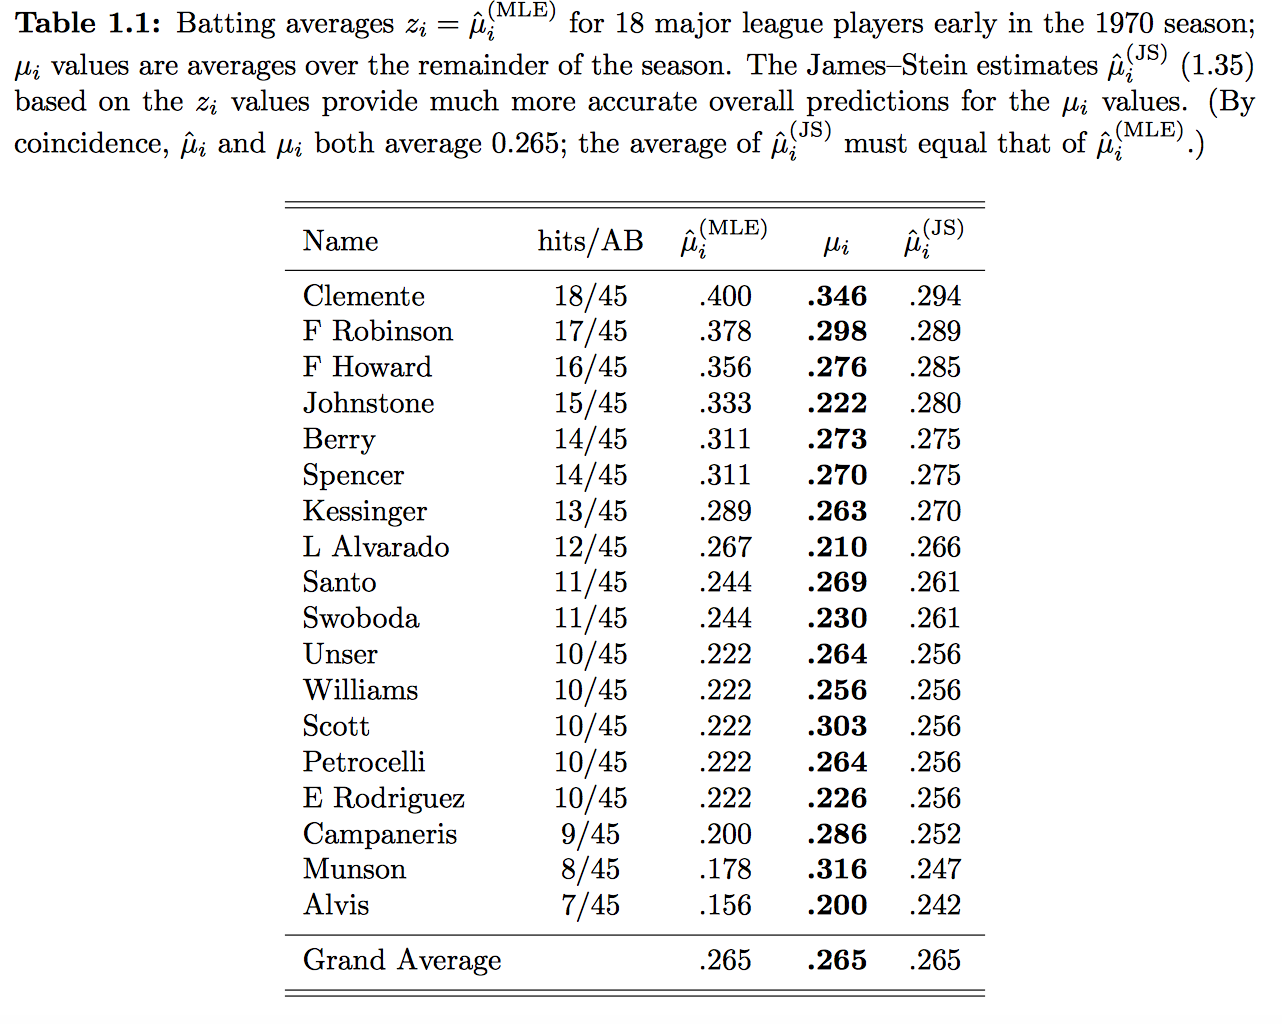
\includegraphics[width=3.5in]{./resources/baseball.png}
\end{center}
\end{frame}

\begin{frame}[fragile]{A (famous) Baseball Example}
Probably we can do better than the MLE here:
\begin{itemize}
\item Thurman Munson wins Rookie of the Year and ends up batting $\mu_i = .316$. If he batted .178 all year, his career would not have lasted long.
\item Clemente's $.400$ seems unlikely to hold up. Last player to hit $> .400$ was Ted Williams $.406$ in 1941.
\item But how?
\end{itemize}
\end{frame}

\begin{frame}[fragile]{Bayesian Shrinkage}
Idea is to take an average between the observed average $y_i$ and the overall mean $\overline{y}$:
\begin{align*}
\widehat{\mu}_i^{JS} &=  (1-\lambda) \cdot \overline{y}  + \lambda \cdot y_i, \quad
\lambda = 1 - \frac{(m-3) \sigma^2}{\sum_i( y_i - \overline{y})^2}
\end{align*}
\begin{itemize}
\item This has the effect of \alert{shrinking} $y_i$ towards the \alert{prior mean} $\overline{y}$.
\item In this case the \alert{prior mean} is just $\overline{y}$ the grand-mean of all players
\item How can information about unrelated players inform us about $\mu_i$?
\item Also consider proportion of foreign cars in Chicago as an additional $y_i$, can this help too?
\item The \alert{shrinkage factor} $\lambda$ depends on sample size and variance, but how is it chosen?
\end{itemize}
\end{frame}



\begin{frame}[fragile]{A Baseball Example}
\begin{center}
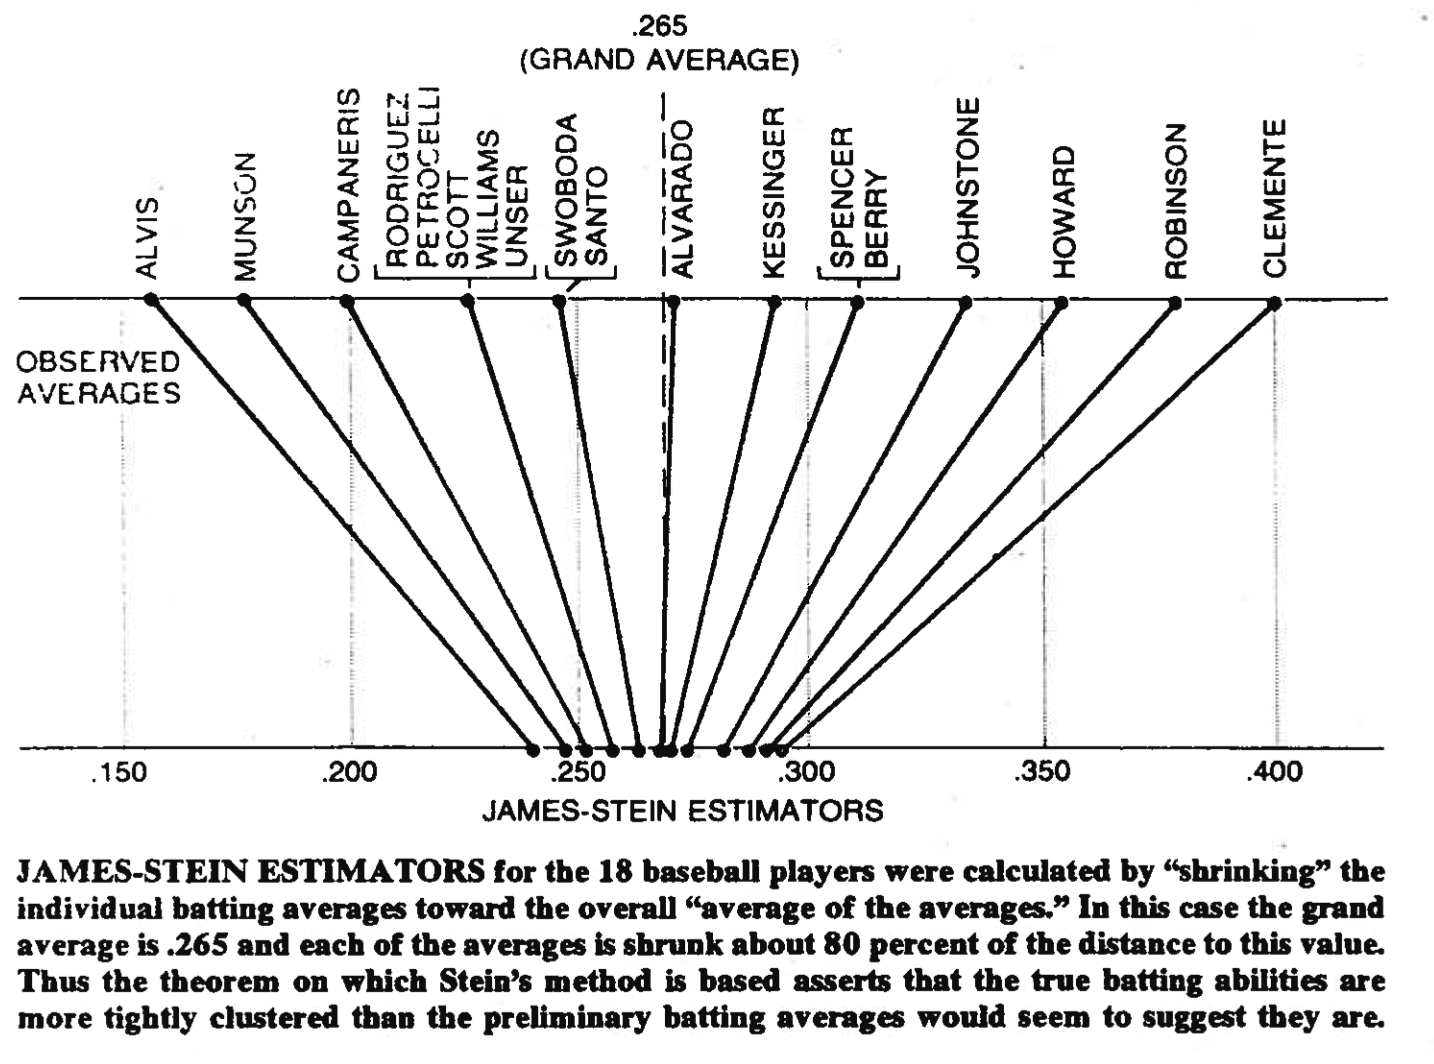
\includegraphics[width=3.5in]{./resources/baseball2.png}
\end{center}
\end{frame}
\section{Example: Diversion Ratios}
\begin{frame}{The Diversion Ratio: Conlon and Mortimer (2018)}
 Raise price of good $j$. People leave. What fraction of leavers switch to $k$?
\begin{eqnarray*}
D_{jk} = \frac{\frac{\partial q_k}{\partial p_j}}{\left|\frac{\partial q_j}{\partial p_j} \right|}
\end{eqnarray*}
It's one of the best ways economists have to characterize competition among sellers.
\begin{itemize}
\item High Diversion: Close Substitutes $\rightarrow$ Mergers more likely to increase prices.
\item Very low diversion $\rightarrow$ products may not be in the same market.\\ (ie: Katz \& Shapiro)
\item Demand Derivatives NOT elasticities.
\item No equilibrium responses.
\end{itemize}
\end{frame}

\begin{frame}
\frametitle{Estimating $\overline{D}_{jk}$}
Remove a product $j$ measure $\Delta q_j$ and $\Delta q_k$.
 \begin{eqnarray*}
 \overline{D_{jk}} =  \frac{\widehat{\Delta q_k}}{|\widehat{\Delta q_j}|} = \frac{ E[q_k | Z=1] - E[q_k | Z=0]}{ \left| E[q_j | Z=1] - E[q_j | Z=0] \right|}  
 =\frac{ E[q_k | Z=1] - E[q_k | Z=0]}{ E[q_j | Z=0] }
 \end{eqnarray*}
\end{frame}

\begin{frame}
\frametitle{Using a Beta-Binomial Prior}
How to restrict $D_{jk} \in [0,1]$?
\begin{eqnarray*}
\Delta q_k | \Delta q_j,D_{jk} &\sim& Bin(n=\Delta q_j, p=D_{jk})\\ \pause
 D_{jk} | \beta_1, \beta_2 &\sim& Beta(\beta_1,\beta_2)\\
E[D_{jk} | \beta_1, \beta_2, \Delta q_j, \Delta q_k] &=& \frac{\beta_1 + \Delta q_k}{\beta_1 + \beta_2 + \Delta q_j}\\ \mu_{jk} &=& \frac{\beta_1}{\underbrace{\beta_1+\beta_2}_{m_{jk}}},  \quad \lambda = \frac{m_{jk}}{m_{jk} + \Delta q_j} \\
\widehat{D_{jk}} &=& \lambda \cdot \mu_{jk} + (1-\lambda) \frac{\widehat{\Delta q_k}}{\widehat{\Delta q_j}}
\end{eqnarray*}
$\mu_{jk}$ is prior mean; $m_{jk}$ is no. pseudo-obs; $\lambda$ weights our prior mean. \\% vs. experimental obs.
When we have a lot of experimental obs, prior receives little weight.
\end{frame}

\begin{frame}
\frametitle{Using a Dirichlet Prior}
How do restrict $D_{j\cdot} \in \Delta$?
\begin{itemize}
\item Same idea as before, but use \alert{Dirichlet Prior}.
\item Acts like pseudo-observations from the \alert{multinomial} distribution.
\item If we had same number of treated observations for each substitute we would have conjugacy/closed form (We don't).
\item Likelihood is $\Delta q_{k} \sim Binomial(\Delta q_j, D_{jk})$ not \alert{multinomial}.
\item We use $m=3.05$ pseudo-observations for the Dirichlet prior.
\item Estimator is still technically \alert{non-parametric}. Why?
\end{itemize}
\end{frame}



\begin{frame}
\frametitle{Shrinkage Estimator, Intuition}
\begin{itemize}
\item We ``shrink'' towards the prior mean when we have experimental estimates that are imprecise.
\item Idea is very simple: when we have lots of data, use the experimental measure.
\item When data are scarce: put more weight on the prior/model-based measure.
\begin{itemize}
\item In practice: FTC/DOJ tend to assume diversion proportional to marketshare
\item Use plain logit (could also use more complicated model)
\item Logit sets the mean of the prior as: $\mu_{jk} = \frac{s_k}{1-s_{j}}$
\end{itemize}
\end{itemize}
\end{frame}

\begin{frame}{Results: Mars }
\tiny
\begin{tabular}{ll |   r r r r  r r r  r}
Firm & Product & \# Weeks & $\Delta q_k$ & $\Delta q_j$ & $\frac{\Delta q_k}{\Delta q_j}$ & Beta(J) & Beta(300) & Dirichlet(4.15)\\ 
\hline  &&\multicolumn{7}{c}{Snickers Removal}\\ \hline
Mars & M\&M Peanut & 176 & 375.52 & -954.30 & 39.35 & 37.04 & 30.80 & 18.40 \\
Mars & Twix Caramel & 134 & 289.60 & -702.39 & 41.23 & 37.86 & 29.49 & 15.88 \\
Pepsi & Rold Gold (Con) & 174 & 161.37 & -900.11 & 17.93 & 16.84 & 13.95 & 7.54 \\
Nestle & Butterfinger & 61 & 72.95 & -362.82 & 20.11 & 17.07 & 11.19 & 4.45 \\
Mars & M\&M Milk Chocolate & 97 & 71.76 & -457.36 & 15.69 & 13.83 & 9.85 & 4.14 \\
Kraft & Planters (Con) & 136 & 78.01 & -759.87 & 10.27 & 9.57 & 7.80 & 3.81 \\
Kellogg & Zoo Animal Cracker & 177 & 65.72 & -970.22 & 6.77 & 6.48 & 5.68 & 2.92 \\
Pepsi & Sun Chip & 159 & 45.30 & -866.09 & 5.23 & 4.98 & 4.33 & 2.07 \\
Hershey & Choc Hershey (Con) & 41 & 29.78 & -179.57 & 16.58 & 12.17 & 6.30 & 2.01 \\
& Outside Good & 180 & 460.89 & -970.22 & 47.50 &  &  & 23.12 \\

\hline  &&\multicolumn{7}{c}{M\&M Peanut Removal}\\ \hline
Mars & Snickers & 218 & 296.58 & -1239.29 & 23.93 & 22.90 & 19.91 & 16.47 \\
Mars & Twix Caramel & 176 & 110.93 & -1014.32 & 10.94 & 10.39 & 8.88 & 6.76 \\
Mars & M\&M Milk Chocolate & 99 & 73.47 & -529.58 & 13.87 & 12.46 & 9.18 & 6.26 \\
Nestle & Raisinets & 181 & 71.82 & -1001.14 & 7.17 & 6.82 & 5.82 & 4.37 \\
Kraft & Planters (Con) & 190 & 61.42 & -1046.10 & 5.87 & 5.62 & 4.90 & 3.60 \\
Hershey & Twizzlers & 62 & 32.98 & -332.99 & 9.90 & 8.32 & 5.32 & 3.35 \\
Kellogg & Rice Krispies Treats & 46 & 22.37 & -220.17 & 10.16 & 7.90 & 4.43 & 2.51 \\
Pepsi & Frito  & 160 & 37.25 & -902.42 & 4.13 & 3.95 & 3.47 & 2.37 \\
& Outside Good& 218 & 606.18 & -1238.49 & 48.95 &  &  & 36.35 \\
\end{tabular}
\end{frame}


\begin{frame}{Results: Kellogg's}
\tiny
\begin{tabular}{ll |   r r r r  r r r  r}
Firm & Product & \# Weeks & $\Delta q_k$ & $\Delta q_j$ & $\frac{\Delta q_k}{\Delta q_j}$ & Beta(J) & Beta(300) & Dirichlet(4.15)\\ 
\hline  &&\multicolumn{7}{c}{Animal Crackers Removal}\\ \hline
Pepsi & Rold Gold (Con) & 132 & 114.39 & -440.80 & 25.95 & 22.90 & 16.21 & 9.89 \\
Mars & Snickers & 145 & 92.44 & -483.63 & 19.11 & 17.26 & 13.04 & 7.58 \\
Mars & M\&M Peanut & 142 & 77.72 & -469.44 & 16.55 & 14.98 & 11.43 & 6.47 \\
Kellogg & CC Famous Amos & 144 & 66.18 & -478.20 & 13.84 & 12.40 & 9.15 & 5.39 \\
Pepsi & Baked Chips (Con) & 134 & 62.55 & -447.60 & 13.97 & 12.46 & 9.13 & 5.27 \\
Mars & Twix Caramel & 110 & 50.17 & -338.97 & 14.80 & 12.75 & 8.74 & 4.58 \\
Sherwood & Ruger Wafer (Con) & 119 & 48.20 & -368.65 & 13.07 & 11.28 & 7.63 & 4.28 \\
Hershey & Choc Herhsey (Con) & 30 & 33.60 & -132.57 & 25.34 & 17.14 & 7.86 & 3.81 \\
Kellogg & Rice Krispies Treats & 13 & 23.52 & -37.80 & 62.22 & 23.24 & 7.16 & 2.99 \\
Kar's Nuts & Kar Sweet\&Salty Mix & 95 & 30.06 & -334.50 & 8.99 & 7.72 & 5.27 & 2.73 \\
Misc & Popcorn (Con) & 56 & 25.72 & -226.89 & 11.34 & 8.92 & 5.08 & 2.61 \\
Kraft & Planters (Con) & 114 & 28.05 & -380.25 & 7.38 & 6.53 & 4.78 & 2.43 \\
Mars & M\&M Plain & 73 & 22.67 & -295.07 & 7.68 & 6.47 & 4.26 & 2.15 \\
& Outside Good& 145 & 240.52 & -482.91 & 49.81 &  &  & 21.98 \\

\hline  &&\multicolumn{7}{c}{Famous Amos Removal}\\ \hline
Pepsi & Sun Chip & 139 & 143.60 & -355.68 & 40.37 & 34.39 & 22.66 & 15.75 \\
Kraft & Planters (Con) & 121 & 82.11 & -332.61 & 24.69 & 20.89 & 13.68 & 8.75 \\
Hershey & Choc Hershey (Con) & 38 & 48.60 & -66.84 & 72.72 & 36.93 & 13.36 & 7.18 \\
Pepsi & Frito & 119 & 49.88 & -313.21 & 15.93 & 13.44 & 8.85 & 5.32 \\
Misc & Rasbry Knotts & 133 & 46.62 & -345.38 & 13.50 & 11.45 & 7.49 & 4.81 \\
Pepsi & Grandmas Choc Chip & 95 & 39.99 & -259.21 & 15.43 & 12.51 & 7.62 & 4.49 \\
Pepsi & Dorito Buffalo Ranch & 72 & 38.11 & -224.24 & 17.00 & 13.28 & 7.53 & 4.43 \\
Pepsi & Chs PB Frito Cracker & 34 & 26.87 & -83.65 & 32.13 & 18.16 & 7.14 & 3.74 \\
Kellogg & Choc Sandwich FA & 57 & 27.97 & -122.04 & 22.91 & 15.06 & 6.84 & 3.69 \\
Pepsi & Rold Gold (Con) & 147 & 32.62 & -392.22 & 8.32 & 7.40 & 5.54 & 3.19 \\
Kraft & Oreo Thin Crisps & 29 & 20.73 & -43.29 & 47.89 & 19.20 & 6.12 & 3.05 \\
Mars & Combos (Con) & 98 & 23.56 & -274.54 & 8.58 & 7.03 & 4.34 & 2.61 \\
& Outside Good& 156 & 192.90 & -399.12 & 48.33 &  &  & 20.95 \\
\end{tabular}
\end{frame}

\begin{frame}{Comparison of Assumptions: Snickers Experiment}
\begin{table}
\footnotesize
\begin{tabular}{|l|ccccc|}
%& Total  & Impose & Impose & Impose & Impose\\ 
\multicolumn{1}{c}{} & \multicolumn{1}{c}{Total} & \multicolumn{1}{c}{Assn 1} & \multicolumn{1}{c}{Assn 2}   & \multicolumn{1}{c}{Assn 3} & \multicolumn{1}{c}{Assn 4} \\ 
\multicolumn{1}{c}{} 	&\multicolumn{1}{c}{} 	&\multicolumn{1}{c}{} 	&\multicolumn{1}{c}{} 	&\multicolumn{1}{c}{($m = K$)} 	&\multicolumn{1}{c}{(m = 4.15)} \\ \hline
Products with $D_{jk} < $ 0 & 51&24&26&0&0\\
Products with $0 \leq D_{jk} \leq 10$& 51&13&15&43&48\\
Products with $10 \leq D_{jk} \leq 20$ & 51&5&5&5&2\\
Products with $D_{jk} > $ 20 & 51&9&5&3&1\\ \hline
Sum of all positive $D_{jk}$s & 51&402.84&301.95&265.41&98.72\\
Sum of all negative $D_{jk}$s & 51&-238.90&-239.07&0.00&0.00\\
\hline
\end{tabular}\\
\footnotesize
Note: Table includes only products for which there were at least 50 sales of the focal product in control weeks, on average.
\end{table}
\end{frame}

\section{Bayesian Estimation}

\begin{frame}{How do we estimate these models?}
A few options
\begin{itemize}
\item With conjugate priors we can closed forms
\item Can do it by hand if we have \alert{sufficient statistics}
\begin{itemize}
\item Clear in beta-binomial or poisson-gamma relationship.
\item Mostly not the case.
\end{itemize}
\item Mostly we do what is known as \alert{Markov Chain Monte Carlo}
\item The goal is to draw from $f(\theta | \mathbf{X})$ or to compute moments of the distribution $E_f[g(\theta)]$.
\end{itemize}
\end{frame}

\begin{frame}{Monte Carlo Methods}
\begin{itemize}
\item Suppose we want to calculate a function 
$$E_f[g(x)] = \int g(x) f(x) d\,x$$
\item How do we do it?
\begin{enumerate}
\item Draw from $\hat{x}_s \sim f(x)$
\item Caclulate $g(\hat{x}_s)$
\item Repeat for $s=1\ldots,S$
\item Calculate $E[\hat{g}]=\frac{1}{S} \sum_{s=1}^S g(\hat{x}_s)$
\end{enumerate}
\end{itemize}
\end{frame}


\begin{frame}[fragile]{Monte Carlo Example}
\begin{itemize}
\item Let's integrate $g(x) = \phi(x)$ (normal pdf) over $f(x) = Unif(0,1)$ from $[0,1]$.
\item We know the answer is $\Phi(1) - \Phi(0)$.
\end{itemize}
\begin{minted}{R}
Integral <- function(n){
    X <- runif(n)
    Y <- exp(-X^2/2)/sqrt(2*pi)
    Int <- sum(Y)/n
    Error <- Int-(pnorm(1)-pnorm(0))
    list(Int,Error)}
\end{minted}
\end{frame}

\begin{frame}{MCMC}
\begin{itemize}
\item Linear regression is nice because it has closed forms (even in Bayesian
framework).
\item In most nonlinear models, it's hard to write down the posterior in
closed form.
\item It's often easier to sample from a distribution than to characterize
it.
\end{itemize}
\end{frame}


\begin{frame}{Gibbs Sampling}
The first building block is known as the \alert{Gibbs Sampler}
\begin{itemize}
\item Suppose that $p(x,y)$ is a p.d.f or p.m.f that is hard to sample directly from.
\item But suppose that $p(x | y)$ or $p(y | x)$ are easy to sample from.
\item Gibbs sampler says:
\begin{enumerate}
\item Initialize $(x_0,y_0)$.
\item Randomly draw $y_1 \sim g(y | x_0)$.
\item Randomly draw $x_1 \sim f(x | y_1)$.
\item Randomly draw $y_2 \sim g(y | x_1)$.
\item Rinse and Repeat. 
\end{enumerate}
\item This sequence $(x_0,y_0),(x_1,y_1), (x_2,y_2), \ldots$ is a \alert{Markov Chain}.
\item Why? Because $(x_k,y_k) | (x_{k-1},y_{k-1})$ doesn't depend on $x_{k-h}$ or $y_{k-h}$ for $h \geq 2$.
\begin{itemize}
\item This does not mean that $(x_3,y_3)$ and $(x_1,y_1)$ are I.I.D!
\end{itemize}
\end{itemize}
\end{frame}

\begin{frame}{Comments}
\begin{itemize}
\item Can prove that the Gibbs sampler converges to the posterior distribution
of $\theta|X,$ regardless of starting value $\theta^{0}$, under
some regularity conditions.
\begin{itemize}
\item In practice, you throw out a chunk of observations at the beginning
of a run as ``burn-in.''
\end{itemize}
\item For any statistic you want to compute, it would suffice to draw from
the posterior distribution of $\left(u,\beta,\Sigma\right)$ and simulate
the statistic at these points.

\begin{itemize}
\item In practice: you pick every $m$th point along your chain.
\end{itemize}
\item No explicit optimization!
\end{itemize}
\end{frame}


\begin{frame}{Bayesian Multinomial Probit}
\begin{itemize}
\item Consider the following model: 
\begin{align*}
u_{ij} & =X_{ij}\beta+\epsilon_{ij}^{*},\ j=1,\ldots,J-1\\
u_{i0} & =\epsilon_{i0}.
\end{align*}
 In matrix form: 
\[
u_{i}=X_{i}\beta+\epsilon_{i},\ \epsilon_{i}\sim N(0,\Sigma).
\]
 We observe 
\[
y_{ij}=1(u_{ij}\geq u_{ik}\forall k),
\]
 as well as $X.$
\end{itemize}
\end{frame}
%
\begin{frame}{Key insight}
\begin{itemize}
\item We want to be able to sample from 
\[
p(\beta,\Sigma|y_{1},\ldots,y_{N},X).
\]
\item If we knew $u$ we could estimate $\beta,\Sigma$ via linear regression.
\item We don't know $u,$ but if we can sample from its marginal distribution
and treat it as data, we can alternate ``regression'' steps and
new draws of $u.$
\end{itemize}
\end{frame}
%
\begin{frame}{McCulloch and Rossi (JoE 1994)}
\begin{itemize}
\item Estimation procedure as follows.
\begin{itemize}
\item Start with a guess of $\beta,\Sigma.$
\item Iterate the following steps:

\begin{enumerate}
\item Draw $u|\beta,\Sigma$, subject to constraints imposed by $y_{i}:$
\end{enumerate}
\begin{itemize}
\item If $y_{ij}=1$ then we must have $u_{ij}\geq u_{ik}$ for all $k\neq j.$
\end{itemize}
\begin{enumerate}
\item With $u$ in hand, derive $\beta,\Sigma$ from posterior distribution
given their priors, $X$, and $u.$ (regression step)
\end{enumerate}
\item Repeating steps (a) and (b) creates a markov chain which converges
to the joint distribution of $\beta,\Sigma,u$.
\item Estimator is an example of a Gibbs sampler.
\end{itemize}
\end{itemize}
\end{frame}
%
\begin{frame}{Estimation outline}
\begin{itemize}
\item Impose Normal and IW priors for $\beta,\Sigma$ respectively.
\item Iterate the following steps:

\begin{itemize}
\item Step 1: $N*J$ conditional distributions $u_{ij}|u_{i,-j},\beta,\Sigma,X,y$
\item Step 2: $\beta|u,\Sigma,X,y$
\item Step 3: $\Sigma|u,\beta,X,y$
\end{itemize}
\item Steps (2) and (3) are exactly as in the multivariate regression model.
\end{itemize}
\end{frame}
%
\begin{frame}{Step 1 details}
\begin{itemize}
\item for each $i,j$, $u_{ij}|u_{i,-j},\beta,G,y_{i}$ is distributed according
to a truncated univariate normal distribution.
\begin{enumerate}
\item If $u=\left[\begin{array}{c}
u_{_{ij}}\\
u_{i,-j}
\end{array}\right]$ is normally distributed with mean $\mu=\left[\begin{array}{c}
\mu_{_{ij}}\\
\mu_{i,-j}
\end{array}\right]$ and variance $\Sigma=\left[\begin{array}{cc}
\Sigma_{jj} & \Sigma_{j,-j}\\
\Sigma_{-j,j} & \Sigma_{-j,-j}
\end{array}\right]$, then 
\[
u_{ij}|u_{i,-j}\sim N(\mu_{ij}+\Sigma_{-j,j}\Sigma_{-j,-j}^{-1} \left( u_{i,-j}-\mu_{i,-j}\right), \ \Sigma_{jj}-\Sigma_{-j,j}\Sigma_{-j,-j}^{-1}\Sigma_{j,-j}).
\]
Here, $\mu=X_{i}\beta.$
\item Truncation points: 

\begin{enumerate}
\item If $y_{ij}=1$, then we know $u_{ij}\geq\max_{k\neq j}u_{ik}.$
\item Otherwise, $u_{ij}\leq\max_{k\neq j}u_{ik}.$
\end{enumerate}
\item To draw from a distribution $F$ truncated at $[l,u]$, draw a uniform
random number $x$ and compute 
\[
u_{ij}=F^{-1}(xF(l)+(1-x)F(u)).
\]
\end{enumerate}
\end{itemize}
\end{frame}
%
\begin{frame}{data augmentation}
\begin{itemize}
\item Treating $u$ as an additional unknown parameter is an example of
\textbf{data augmentation}.
\item Well-chosen auxiliary parameters can make Bayesian estimation tractable.
\item Try augmenting the data with $\epsilon\equiv u-X\beta$ instead of
$u$! 
\end{itemize}
\end{frame}
%
\begin{frame}{When does Gibbs sampling fail?}
\small
\begin{example}[High-probability island ]
Let 
\[
S=\{0,1\}^{100}.
\]
Suppose that the zero vector has probability $P(0)=1/2$, and all
other vectors are equally likely, i.e. occur with probability $P(s)=\frac{1}{2}\cdot\frac{1}{2^{100}-1}.$ 

Consider a Gibbs sampler with an initial value of $s=0$. Suppose
that we are updating the $j$th component. There are two possible
outcomes, $e_{j}$ and $0.$ We have:
\begin{align*}
p(e_{j}|0) & =\frac{1}{2^{100}-1}/\left(\frac{1}{2^{100}-1}+1\right)\approx\frac{1}{2^{100}}\\
p(0|0) & =1/\left(\frac{1}{2^{100}-1}+1\right)\approx1.
\end{align*}
 
\end{example}
Once $0$ is reached, it will take approximately $2^{100}$ draws
on average to draw a value other than $0.$ Therefore it will take
{*}many{*} draws to estimate $P(0).$ 
\end{frame}
%
\begin{frame}{When does Gibbs sampling fail?}
\footnotesize
Another failure mode occurs when there are multiple high-probability
islands.
\begin{example}[Two islands ]
Let 
\[
S=\{0,1\}^{2}.
\]
 and suppose 
 {\footnotesize
\begin{align*}
P(0,0) & =\frac{1}{2}\\
P(1,1) & =\frac{1}{2}\\
P(0,1) & =0\\
P(1,0) & =0.
\end{align*}
}
 In this case a sampler that starts at $(0,0)$ or $(1,1)$ will never
reach the other high-probability state.
\end{example}
\begin{itemize}
\item This example is an extreme case.
\item But Gibbs samplers may mix poorly when the underlying
density has multiple separated peaks.
\end{itemize}
\end{frame}


\begin{frame}{Hierarchical models}
\begin{itemize}
\item Bayesian approach to random effects and random coefficients.
\begin{itemize}
\item Actually much more general than this.
\item Hierarchical models have some parameters that are distributed according
to distributions which in turn have priors.
\end{itemize}
\item Example (random coefficients, McCulloch and Rossi): In the multinomial
probit model, we could impose structure on the covariance matrix as
follows: 
\begin{align*}
u_{i} & =X_{i}\beta_{i}+\epsilon_{i}\\
\epsilon_{i} & \sim N(0,I)\\
\beta_{i} & \sim N(\overline{\beta},\Sigma_{\beta_{i}})\\
\overline{\beta} & \sim N\left(\overline{\overline{\beta}},\Sigma_{\overline{\beta}}\right)\\
\Sigma_{\overline{\beta}} & \sim IW(\alpha,\nu).
\end{align*}
 In this case, $\beta_{i}$ are normally-distributed random coefficients.
The parameters of $F(\beta_{i})$ in turn have prior distributions.
\end{itemize}
\end{frame}
%
\begin{frame}{Random coefficients: estimation}
\begin{itemize}
\item Augment data w/ random coefficients $\beta_{i}$ as well as $u_{i}.$
\item Use Gibbs sampler:
\begin{itemize}
\item Update $u|\beta_{i},X$ exactly as before, except that variance of
$\epsilon$ is fixed at $N(0,I).$ 
\item Update $(\beta_{i}|u,\overline{\beta},\Sigma_{\beta_{i}},X_{i})$,
one observation $i$ at a time.
\item Update $\overline{\beta},\Sigma_{\beta_{i}}|\left\{ \beta_{i}\right\} _{i=1,\ldots,N}$
as in Bayesian linear regression. 
\end{itemize}
\item See McCulloch and Rossi for estimation procedure.
\end{itemize}
\end{frame}
%
\begin{frame}{Metropolis-Hastings}
\begin{itemize}
\item Gibbs samplers require you to know conditional densities.
\item Often, all you know is a function that is proportional to the (conditional)
density.
\begin{itemize}
\item Example: you want to draw from $f(x|x\in R)$ for some region $R$,
and you know $f(x)$, but it is difficult to characterize the region
$R.$
\item In this case it's easy to compute $f(x)\cdot1(x\in R)$ but difficult
to compute $\frac{f(x)1(x\in R)}{\int_{R}f(x)dx}.$ 
\end{itemize}
\item Metropolis-Hastings simulators are algorithms to sample from a density
when you know a function proportional to it.
\item You can even use MH for conditional distributions within a Gibbs sampler
(known as MH-within-Gibbs).
\end{itemize}
\end{frame}
%
\begin{frame}{MH algorithm}
\begin{itemize}
\item Suppose you know a function $\pi(x|data)$ which is proportional to $f(x|data).$
\item The Metropolis-Hastings simulator creates a sequence that converges
to the stationary distribution $\pi(\cdot).$
\item Algorithm is as follows:
\begin{enumerate}
\item Fix a proposal density $q(x'|x).$ 
\item Start at $x=x^{(0)}.$ 
\item For iteration $i=1,\ldots,T$ do:
\begin{itemize}
\item Propose $x'\sim q(x'|x^{(i-1)})$
\item Define the acceptance probability 
\[
\alpha(x'|x)=\min\left\{ 1,\frac{q(x'|x^{(i-1)})\pi(x'|data)}{q(x^{(i-1)}|x')\pi(x^{(i-1)}|data)}\right\} .
\]
\item Update $x$ according to: 
\[
x^{(i)}=\begin{cases}
x' & \text{ with probability }\alpha(x'|x)\\
x^{(i-1)} & \text{ with probability }1-\alpha(x'|x)
\end{cases}.
\]
\end{itemize}
\end{enumerate}
\end{itemize}
\end{frame}
%
\begin{frame}{Choosing a proposal density}
\begin{itemize}
\item Symmetric proposal density 
\[
q(x'|x)=q(x|x')
\]
 is a popular choice. 
\begin{itemize}
\item This option is known as \textbf{random walk Metropolis-Hastings}.
\item Normal distribution is a popular choice within this class: 
\[
q(x'|x)=\phi(x'-x;\ 0,\sigma_{q}^{2}).
\]
\item For any symmetric $q(\cdot|\cdot)$:
\[
\alpha(x'|x)=\min\left\{ 1,\frac{\pi(x'|data)}{\pi(x|data)}\right\} .
\]
\item Aim for acceptance rate$\approx1/3$ by choice of scale of proposal
distribution? 
\begin{itemize}
\item Too low and too many draws are needed.
\item Too high and the chain mixes slowly.
\end{itemize}
\end{itemize}
\end{itemize}
\end{frame}
%
\begin{frame}{Other proposal densities}
\begin{enumerate}
\item Independent proposal density: 
\[
\alpha(x'|x)=\min\left\{ 1,\frac{q(x')\pi(x'|data)}{q(x)\pi(x|data)}\right\} .
\]

\begin{itemize}
\item Can be convenient if some choice of $q(\cdot)$ is easy to sample
from \textbf{and }results in an easy-to-evaluate expression for $q(x)\pi(x).$ 
\end{itemize}
\item Other proposal densities that simplify the expression $\frac{q(x'|x^{(i-1)})\pi(x'|data)}{q(x^{(i-1)}|x')\pi(x^{(i-1)}|data)}$.
\end{enumerate}
\end{frame}
%
\begin{frame}{Other methods when your ``density'' doesn't integrate to 1}
\begin{itemize}
\item MH is not the only method for sampling when all you know is a function
proportional to the density.
\item Slice sampling (Neal 2003) can be practical on some problems.
\item Also: Hamiltonian Monte Carlo (aka ``Hybrid Monte Carlo'')
\begin{itemize}
\item Requires gradient, but can be much faster to converge than MH.
\end{itemize}
\end{itemize}
\end{frame}
%
% \begin{frame}{Slice sampling}
% \end{frame}
% %
\begin{frame}{Hamiltonian Monte Carlo}
Hamiltonian Monte Carlo combines ideas from physics with the Metropolis-Hastings algorithm to sample from the posterior with much less autocorrelation than random-walk MH algorithms.

My slides follow Neal (2012), ``MCMC using Hamiltonian Dynamics''
\end{frame}

\begin{frame}{Hamiltonian}
Think of a marble rolling around on a surface.  The marble has:
\begin{itemize}
	\item a $d$-dimensional position vector, $q$
	\item a $d$-dimensional momentum vector, $p$
\end{itemize}
Define the {\it Hamiltonian} as follows:
$$  H(q,p) = U(q) + K(p)  $$
where
\begin{itemize}
	\item $U(q)$ is the potential energy (depends on position).
	\item $K(p)$ is the kinetic energy (depends on how fast the marble is moving).
\end{itemize}
\end{frame}

\begin{frame}{Hamiltonian dynamics}
The partial derivatives of the Hamiltonian determine how $p$ and $q$ evolve.
\begin{align*}
\frac{\partial q_i}{\partial t} &= \frac{\partial H}{\partial p_i} \\
\frac{\partial p_i}{\partial t} &= -\frac{\partial H}{\partial q_i} 
\end{align*}
These equations imply that the Hamiltonian is invariant.
\end{frame}

\begin{frame}{Details}

$$H(q,p) = U(q) + K(p)$$

\begin{enumerate}
	\item Typically, $K(p) = p'M^{-1}p/2$, where $M$ is a symmetric, positive-definite ``mass matrix''.  (This is the formula for kinetic energy.)
	\item Observe that $K(p)=p'M^{-1}p/2$ is also the log-pdf of a Normal with mean 0 and covariance $M$.
	\item In physics, $U(\cdot)$ would represent the height of the surface at different locations.
	\item We're going to choose $U(\cdot)$ to have a probabiliistic interpretation.
\end{enumerate}
\end{frame}

\begin{frame}{Interpretation as probability}
\begin{itemize}
	\item Fact (from statistical mechanics): Given a ``temperature'' $T$, Hamiltonian dynamics imply a joint distribution of states, given by 
$$ Pr(q,p) = \frac{1}{Z}\exp\left( \frac{-H(q,p)}{T} \right) $$
\begin{itemize}
	\item  $Z$ is the constant needed to make $Pr(\cdot)$ integrate to 1. \end{itemize}
	\item In our case, taking $T=1$, we have $$Pr(q,p) = \frac{1}{Z}\exp\left( -U(q) \right)\exp\left( -K(p) \right).$$
	\item Goal: pick $U(\cdot)$ so that the marginal of $Pr(\cdot)$ is the posterior over $q$.
	\item Achieve this by picking $$U(q) = -\log \left( \pi(q) L(q|D) \right)$$ where: \begin{itemize}
		\item $\pi(q)$: prior density
		\item $L(q|D)$: likelihood given data $D$.
	\end{itemize}
\end{itemize}
\end{frame}

\begin{frame}{Hamiltonian Monte Carlo algorithm}
Assume \begin{enumerate}
\item prior $\pi(q)$ on parameters $q$
\item Gaussian prior w/ diagonal covariance matrix on $p$, {\bf independent of} $\pi(\cdot)$
\item diagonal mass matrix.
\end{enumerate}
Iterate as follows:
\begin{enumerate}
	\item[0] At beginning of iteration $t$, algorithm has state $(q_t,p_t)$.
	\item[1] Draw a new $p$, iid, from independent Gaussian distribution.  Consider state $(q_t,p)$.
	\item[2] Simulate a trajectory using Hamiltonian dynamics.  Arrive at $(q',p')$.
	\item[3] Use the (standard) Metropolis-Hastings acceptance rule for a symmetric proposal density: 
	$$ \alpha = \min[1, \exp(-H(q',p') + H(q_t,p_t))].$$
	With probability $\alpha$, the new state is $(q',p')$; otherwise it's $(q_t,p_t)$ again.
\end{enumerate}
\end{frame}

\begin{frame}{Simulating Hamiltonian dynamics}
\begin{itemize}
	\item Hamiltonian is conserved under (continuous) Hamiltonian dynamics.
	\item To implement on a computer, need to discretize.  Some subtlety to simulation/discretization. 
	\item Naive methods could cause simulation errors to blow up.
	\item Use ``leapfrog'' algorithm or refinements thereof.  This algorithm keeps Hamiltonian (exactly) constant.  See details in Neal (2012).
\end{itemize}
\end{frame}

\begin{frame}{Hamiltonian Monte Carlo: comments}
\begin{enumerate}
	\item Equations of motion involve gradient of log-likelihood.  Need to provide this.
	\item Why is the proposal density symmetric?  Can prove that ``forward'' trajectory is as likely as ``backward''.
	\item If we skipped step (1), would always have $H(q_t,p_t) = H(q',p')$.  Only change in likelihood of $(p,q)$ comes from new momentum draw in step (1).
	\item Step 1 is necessary. If total energy is fixed, particle will never reach states with likelihood below a given finite value.)
	\item Well-tested implementation in \texttt{STAN} (domain-specific language; callable from \texttt{R/Python/Julia}; provides automatic differentiation).  Fantastic if you can phrase your problem in its language.
	\item If you can shoehorn your problem into \texttt{STAN}, do it!
\end{enumerate}
\end{frame}


\begin{frame}[fragile]{Stan Code}
\footnotesize
\begin{verbatim}
% Main Specification: Dirichlet Prior
data {
  int<lower=1> J;               // number of products, including outside good
  int<lower=1> N[J];            // number of trials
  int<lower=0> y[J];            // number of successes for each product j
  vector[J] priors;    // mean of the distribution of alpha
}

parameters {
  simplex[J] theta;
}

model {
  theta ~ dirichlet(priors);
  for (j in 1:J) {
    y[j] ~ binomial(N[j], theta[j]);
  }
}
\end{verbatim}
\end{frame}




\begin{frame}{An MCMC approach to classical estimation (Chernozhukov and Hong, JoE
2003)}
\begin{itemize}
\item It turns out that MCMC can be useful outside of Bayesian framework.
\item CH consider case of extremum estimation
\begin{itemize}
\item Review: want to maximize a criterion function $L_{n}(\theta)$, where
$n$ is sample size. 
\item Leading example: GMM 
\[
L_{n}(\theta)=-\frac{1}{2}\left(n^{-1/2}\sum_{i=1}^{n}m_{i}(\theta)\right)^{'}W_{n}(\theta)\left(n^{-1/2}\sum_{i=1}^{n}m_{i}(\theta)\right)
\]
 for moment function $m_{i}(\theta)$, weight matrix $W_{n}(\theta).$ 
\end{itemize}
\end{itemize}
\end{frame}
%
\begin{frame}{Laplace-type estimators}
\begin{itemize}
\item Consider an objective function $L_{n}(\theta)$.
\item Pick a prior $\pi(\theta)$ strictly positive and continuous over
$\Theta.$ 
\item The following transformation is known as a\textbf{ quasi-posterior:}
\[
p_{n}(\theta)\equiv\frac{\pi(\theta)\exp(L_{n}(\theta))}{\int_{\Theta}\pi(\theta)\exp(L_{n}(\theta))d\theta}.
\]
\item Quasi-posterior mean is an example of a \textbf{Laplace-type estimator}:
\[
\int_{\Theta}\theta p_{n}(\theta)d\theta
\]

\begin{itemize}
\item Formally: LTEs solve
\[
\hat{\theta}=\arg\inf_{\zeta}\int\rho_{n}(\theta-\zeta)p_{n}(\theta)d\theta
\]
\item Different choices of $\rho_{n}$ give posterior means, medians, $\tau th$
quantiles.
\end{itemize}
\end{itemize}
\end{frame}
%
\begin{frame}{Computing LTEs}

\[
p_{n}(\theta)\equiv\frac{\pi(\theta)\exp(L_{n}(\theta))}{\int_{\Theta}\pi(\theta)\exp(L_{n}(\theta))d\theta}.
\]

\begin{itemize}
\item Even if $L_{n}(\theta)$ is not a likelihood, $p_{n}(\cdot)$ is a
proper density over $\Theta.$ 
\item Goal: compute mean.
\item Can do so via MCMC: 
\[
\hat{\theta}=\frac{1}{B}\sum_{i=1}^{B}\theta^{(i)}
\]
\item In practice:
\begin{itemize}
\item Constant term $\int_{\Theta}\pi(\theta)\exp(L_{n}(\theta))d\theta$
may be difficult to compute.
\item Use Metropolis-Hastings with $f(\theta)=\pi(\theta)\exp(L_{n}(\theta)).$ 
\end{itemize}
\end{itemize}
\end{frame}
%
\begin{frame}{Notes on LTEs}

\[
p_{n}(\theta)\equiv\frac{\pi(\theta)\exp(L_{n}(\theta))}{\int_{\Theta}\pi(\theta)\exp(L_{n}(\theta))d\theta}.
\]

\begin{enumerate}
\item If $L_{n}(\cdot)$ is log-likelihood, then $p_{n}(\theta)$ is the
(Bayesian) posterior.
\item Paper gives two procedures for inference.
\begin{enumerate}
\item Can estimate variance along your sequence, use delta method.
\item Under stronger conditions, to estimate a 95\% CI, can use quantiles
of sequence $\theta^{(i)}.$
\begin{enumerate}
\item Valid in GMM iff you use best estimate of optimal weight matrix. 
\item See paper for details.
\end{enumerate}
\end{enumerate}
\end{enumerate}
\end{frame}


\section*{Thanks!}
\end{document}

\item We probably are interested in more observations $[x_1,\ldots,x_n]$ instead of just $x_1$.
\item $\sum_{i=1}^N x_i \sim Bin(N,p)$.